\documentclass[conference]{IEEEtran}

\usepackage{datetime}
\usepackage{cite}
\usepackage[pdftex]{graphicx}
\usepackage{epstopdf}
\usepackage[utf8]{inputenc}
\usepackage{amsfonts}
\usepackage{amssymb}
\usepackage{graphicx}
\usepackage{tikz}
\usepackage{float}
\usepackage{color}
\usepackage{subfig}
\usepackage[hyphens]{url}

\hyphenation{}

\newcommand{\xcloud}{x-cloud }

\begin{document}

\title{\xcloud challenges}


% author names and affiliations
% use a multiple column layout for up to three different
% affiliations
\author{
\IEEEauthorblockN{Jakub Krzywda}
\IEEEauthorblockA{Dept. of Computing Science\\Umeå University\\
SE-901 87 Umeå, Sweden\\
Email: jakub@cs.umu.se}
\and
\IEEEauthorblockN{William Tärneberg}
\IEEEauthorblockA{Dept. of Electrical and Information Technology\\Lund University\\
Ole Römers väg 3, 223 63 Lund, Sweden \\
Email: william.tarneberg@eit.lth.se}}

\maketitle


\begin{abstract}
%\boldmath
The abstract goes here.
\end{abstract}

\IEEEpeerreviewmaketitle


\section{Introduction}
\begin{figure}[tb]
	\centering
	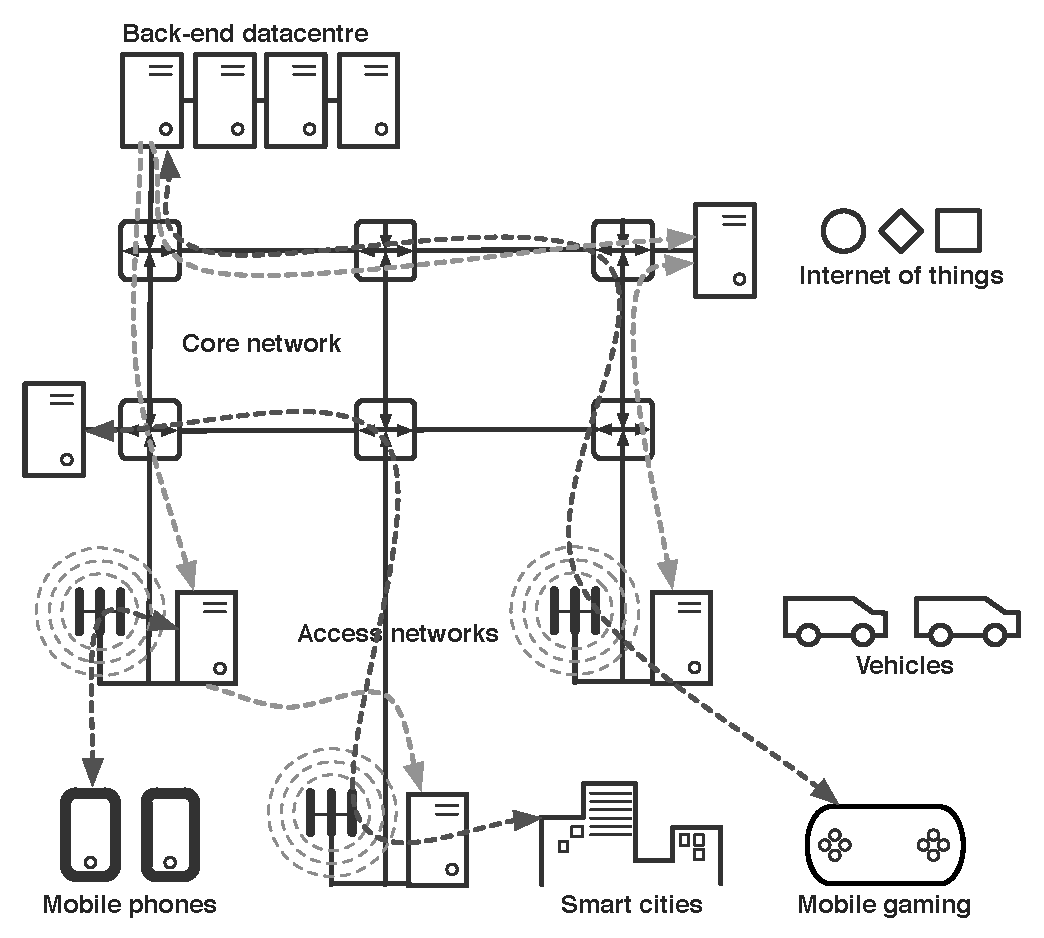
\includegraphics[width=\linewidth]{diagram_overview.pdf} 
	\caption{\xcloud}
	\label{fig:diagram_overview}
\end{figure}

%------------------------------------------------------------------

\section{The case for the \xcloud}

\subsection{The bandwidth case for \xcloud}
\begin{itemize}
\item Internet structure, latency, and bandwidth: \cite{Ramasubramanian:2009:TIL:2492101.1555357}
\end{itemize}

\subsection{The latency case for \xcloud}
The intermediate latency between a client and a data centre is a product of propagation, modulation, and network routing and traffic shaping. Propagation is a clear physical obstacle to reducing latency, and there is very little evidence to suggest that information will propagate faster than $\frac{2}{3}$ of the speed of light, at scale, in the near future. Furthermore, the delay in the backbone network is incurred to the most part by routing. A full point to point network where the propagation speed is the only limit, is not economically viable and would dissolve the fabric of the Internet. As such, we can always expect a certain amount of network contributed latency and jitter. At best, an LTE mobile access network adds about 5 ms of latency \cite{blajic2006latency}. Radio access network latency can be expected to diminish over the next few generations of mobile networks. 

\begin{figure}[tb]
	\centering
	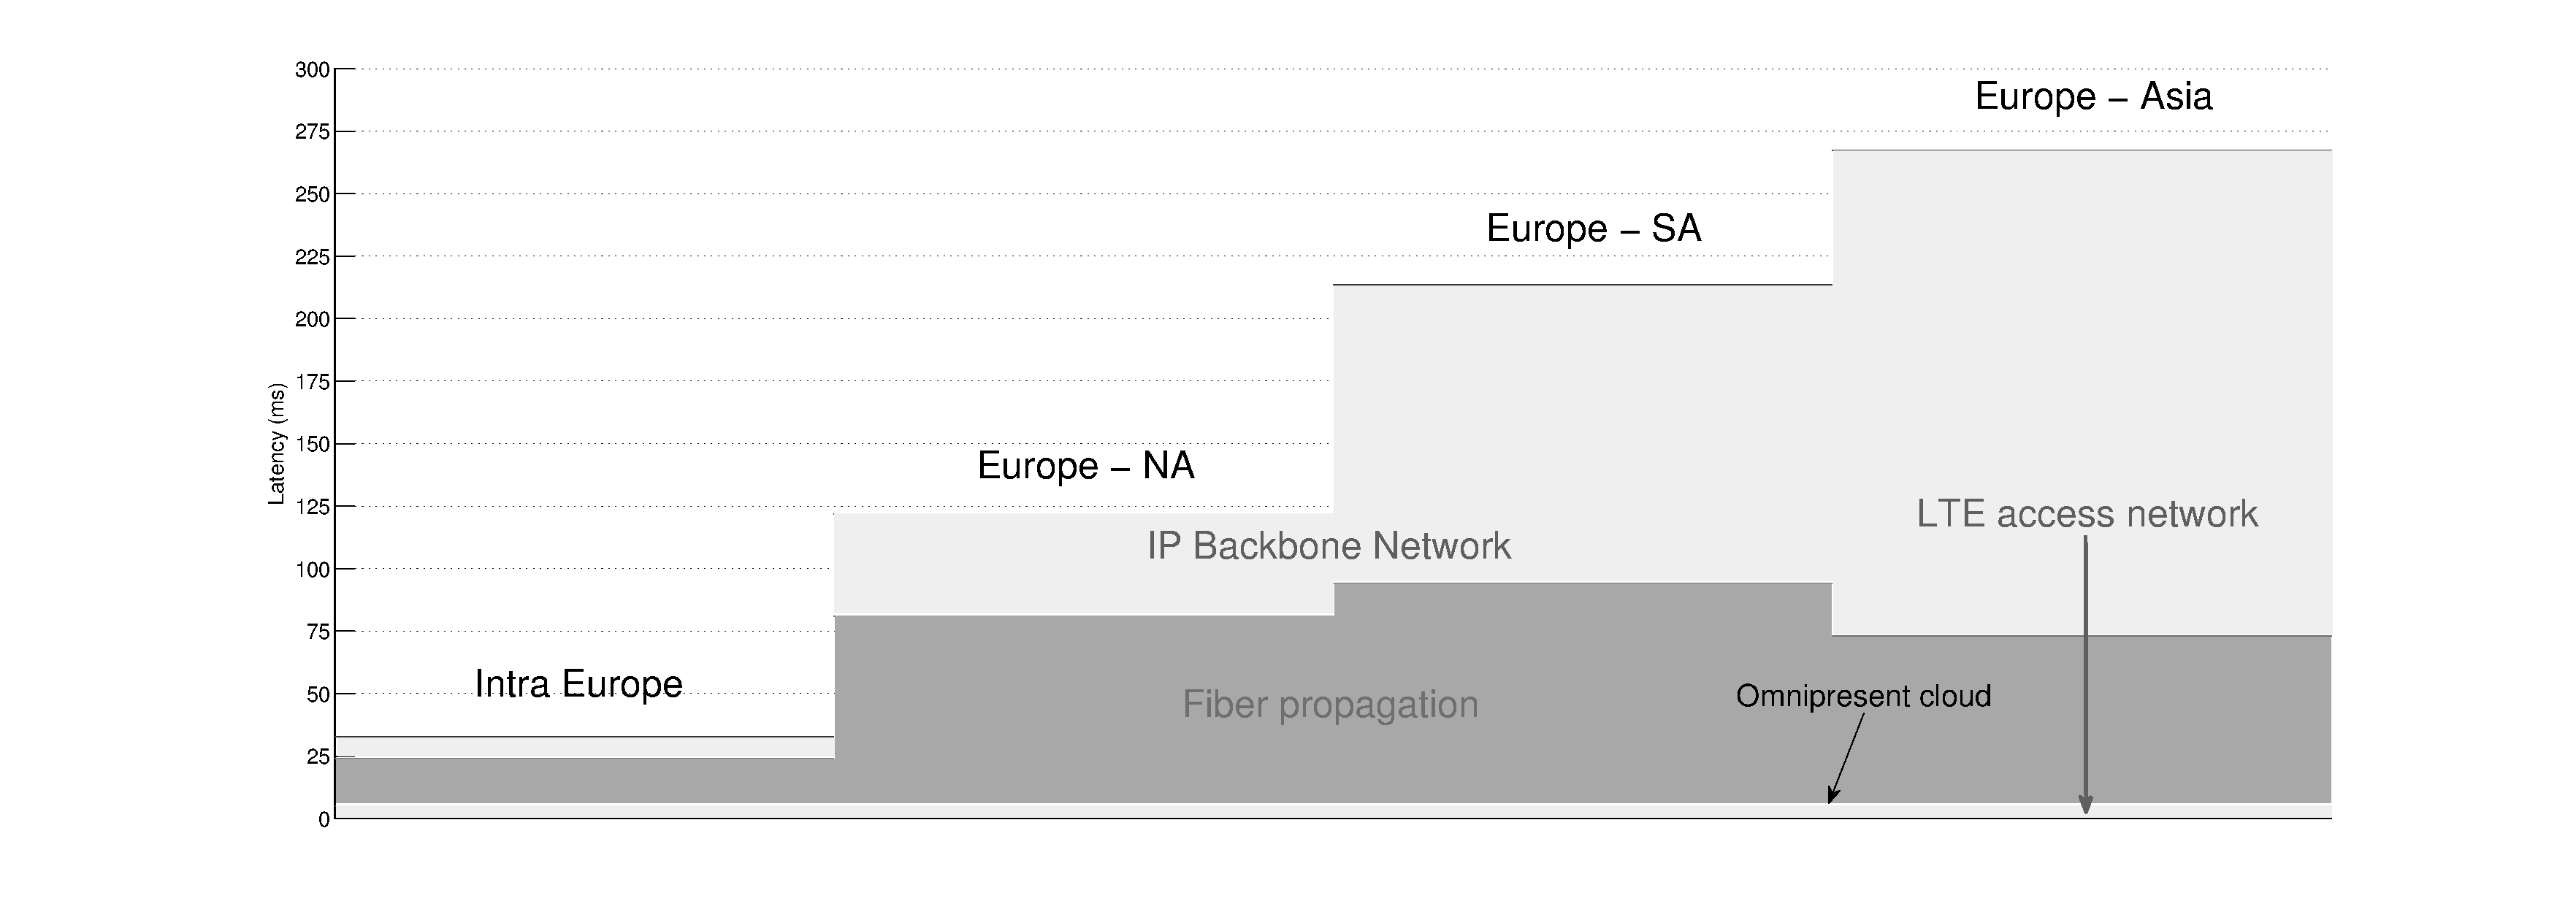
\includegraphics[height=0.12\paperheight]{omni_motivation.pdf} 
	\caption{IP Internet latency in western Europe \cite{BT_IP} over LTE \cite{blajic2006latency}}
	\label{fig:omni_motivation}
\end{figure}

Moving the cloud data centres closer to the IP backbone networks eliminates some of the additive latency on one side of the connection. Doing so, not only eliminate the propagation delay, but will over time, add more complexity to peripheries of the backbone as more severs nodes make their home there. 

The \xcloud remedies this latency challenge in a more sustainable way. By moving compute resources to the mobile networks, IP backbone network propagation and routing delays are eliminate without disrupting the Internet topology. The resulting distributed infrastructure is capable of delivering content and services at latencies less than 10 ms. 

The \xcloud will thus enable latency-sensitive services to be migrated to the cloud, such as, gaming, financial trading, process control, and most real-time human-machine interaction process.

\subsection{The infrastructure case for \xcloud}
Distributed virtualized mobile networks will rely on centralized compute nodes for higher level link management. One node will proposedly host multiple base stations, to which they connect over a network link, much like the Ericsson Radio Dot System \cite{ericsson_dot}, but at a larger scale. The size of these virtualization resource nodes is proportional to the maximum distance they can reside from the radio nodes, given the induced propagation delay. Supposedly these virtualization resource nodes will the placed in the vicinity of the core IP network. The virtualization resource nodes can be seen as to define geographic areas whos boundaries are defined by the reach of the mobile network which it serves. Depending on the level of desired provision and load balancing flexibility, these geographic domains will overlap to varying degrees.

The virtualization resource nodes are conceivably constructed of generic x86 or ARM servers, hosting VMs or containers within which the virtualized mobile network infrastructure is executed. Given the placement of the virtualization resource node, any free or designually excess capacity can be used hist other services.

The topology is designed to optimize the use of radio resources, the geographic domains which the virtualization resource nodes constitute do not necessarily overlap or map the demographic area which \xcloud services operate.

%------------------------------------------------------------------

\section{Proposed research topics}
\subsection{Placement of edge data centres \emph{Ericsson}}
\subsubsection{Proposed research}
There are no clear directions as to what degree the coming mobile networks will be virtualized. The degree of virtualization will determine the distribution of compute resources in the network, bounded by properties such as propagation delay, and cell resource provisioning. ...
\subsubsection{Related research}


\subsection{VM placement and migration decisions \emph{Umeå}}
\subsubsection{Proposed research}
In the \xcloud a service will either exists only locally or distributed, but purposely serves a geographically and demographically bounded populous. The units on which the service is hosted are of limited capacity and cannot he universally virtualized as a traditional data center, with relatively unlimited capacity over time. Give the load on each of the nodes and their geographic relevance to the demographic populous they server, services will conceivably need to be mobile, migrating, dispersing, and contracting to minimize such properties as cost, load, and traffic, also taking into account the cost of the migration itself.

We propose research into an appropriate centralized or distributed, load balancing cost function, taking into account :

\begin{itemize}
\item Incurred migration load on host and receiver
\item Incurred migration induced network congestion
\item Network congestion
\item Delay \/ RTT to client to aggregate client base. In other words, minimize delay to aggregate delay/latency to all its served clients. \emph{Perhaps separate research topic preceding this one}
\item Client mobility
\end{itemize}

A property such as energy consumption is perhaps irrelevant to a topology of small data centres as domain of movement is fairly limited and bounded by the demographic service, the rate of which a service migrates is to some extent bounded by the mobility of its users. Nevertheless, energy can become a relevant parameter if the service is allowed to migrate between the \xcloud and a traditional data centre or if the energy profiles of the local \xcloud hosts, is heterogeneous. As the serviced domain is bounds each service by its sociogeographic profile and the fact that latency gains are fairly small accounting for thermal emissions and reuse would be counter productive, and should be dealt with optimally by each node independently. When optimizing for latency, inherent thermal efficiency will conceivably seldom correlate with the service sociogeographic domain. 

\subsubsection{Related research}
Existing research in this area is mainly focuses on load balancing and provisioning between larger distributed data centres with static users.


\subsection{How many devices can be handle by the current infrastructure (latency/bandwidth limits or other requirements) \emph{Umeå} }
\subsubsection{Proposed research}
The number of devices accessing the cloud services is bound to grow significantly with the advent of the internet of things. Most of these devices will communicate over the mobile network. Although the added devices will not necessarily contribute as much data traffic as a user-interaction device, they will significantly add to the congestion to the radio access networks and the adjacent core network. In such a case the, the congestion might result in increased latency in the mobile access network and the adjacent core network.
\subsubsection{Related research}


\subsection{Influence of huge number of (mobile) devices and internet of things \emph{Umeå} }
\subsubsection{Proposed research}
\subsubsection{Related research}


\subsection{Size of edge data centres (number of CPU, memory, etc.) \emph{Ericsson}}
\subsubsection{Proposed research}
\subsubsection{Related research}


\subsection{What type of traffic should be directed to edge data centres? \emph{Lund}}
\subsubsection{Proposed research}
\subsubsection{Related research}


\subsection{Topology of mobile network (antennas detached from BTS) CRAN \emph{Lund}}
\subsubsection{Proposed research}
\subsubsection{Related research}


\subsection{How mobility of user affects network and cloud computing? \emph{Lund}}
\subsubsection{Proposed research}
\subsubsection{Related research}

%------------------------------------------------------------------

\section{Simulation}

\subsection{Constituent models}
\subsubsection{Data Centre}
Cloud model : \cite{5959161}
Web serve model : \cite{1191656}

\subsubsection{Radio access network}
Because the mobile access network is a service access qualifier, the mechanisms of the network is relatively irrelevant to the primary research topics. The network can appropriately be modelled with a series of delays. 

It is a constituent objective of our research to determine relevant X-Cloud/NGN \footnote{Next Generation Network} symbiotic topologies. These topolgies will be feed into the simulation model and will conceivably encompass, resource placement and dimension, cell sizes, and radio resource provisioning \cite{kwan2010mobility,racz2007handover,salo2010practical}.

Our basic research topics will require a homogeneous, equidistant, and equirange cell topology. Although it is reasonable to assume that future networks hosting an X-Cloud will be distributed. 

\subsubsection{Base station}
The base station can conceivably be modelled with a queue and a delay proportional to its propagation distance to its associated "C-RAN" node.

\subsubsection{Core network}
The essential property of the core network is bandwidth and delay. Both of which can be modelled with queues.

\begin{itemize}
\item Latency
\begin{itemize}
\item "Point-to-Point" core network delay model \cite{choi2007analysis}
\item "One-hop" core network router queue delay model  \cite{papagiannaki2003measurement}
\end{itemize}
\end{itemize}

\subsubsection{Mobility}
A smooth random walk, unobstructed, bounded, edge-aware mobility model will provide a uniformly distributed dispersion of users across the simulation domain \cite{Bettstetter:2001:SBS:381591.381600}. The model is two-dimensional and provides pedestrian, bicycle, and auto mobile mobility modes. The model is uniform and does thus not take into account any socio-demographic variations, and local clusters. Nevertheless, exploring specific demographic and urban settings is beyond the scope of our basic research topics. Furthermore, in the absence of a socio-demographic and urban scenarios, an aggregate mobility mode will be deployed.

\subsubsection{Service}
There is a multitude of appropriate service models. 

Web browsing behaviour : \cite{liu2010understanding}
3-Tiered model : \cite{1521145}
Cloud service usage patterns : \cite{zhao2009cloud}

\subsection{Simulation framework}
Below are the candidate simulation tools and frameworks proposed during the third Cloud Control Workshop. \cite{zhao2012modeling}

\subsubsection{SimJava}

\subsubsection{SimPy}
Python and SimPy has the ability to run powerful statistical analyses with R \cite{rproject}, interact with a MATLAB workspace \cite{pymatlab}, and bind NS-3 modules \cite{ns3python}. Nevertheless, not able to confirm weather or not you can call uncompiled MATLAB SimEvent modules.

\subsubsection{LTE-Sim}
\cite{5634134}

\subsubsection{CloudSim} \cite{cloudsim}

CloudSim adaptations:
\begin{itemize}
\item NetworkCloudSim \cite{6123487}
\item CloudAnalyst \cite{wickremasinghe2010cloudanalyst}
\end{itemize}

\subsubsection{GreenCloud}
\cite{greencloud}

\subsubsection{iCanCloud}
\cite{icancloud}

\subsubsection{MDCSim}
\cite{5289159}

\subsubsection{SimGrid} 
\cite{simgrid}

\begin{itemize}
\item \cite{4488918}
\item \cite{bobelin2012scalable}
\end{itemize}

\subsubsection{CoolSim}
\cite{coolsim}

\subsubsection{ns-3}
\cite{ns3}

\subsubsection{Matlab+SimEvent} (and TrueTime)

%------------------------------------------------------------------

\section{Papers}

\subsection{Comparison of existing simulators from the perspective of  \xcloud}
A survey of existing simulators with comparison of their capabilities (and limitations) to simulate \xcloud.

Simulators of:
\begin{itemize}
\item Data centers,
\item BTS,
\item Network (BTS --- DC),
\item Mobile network,
\item Mobile devices,
\item Users (mobility).
\end{itemize}

What is different in operation/simulation of \xcloud?

\subsection{Limitations of current infrastructure \& the setup/structure of \xcloud}
\subsubsection{Limitations of current infrastructure}
Simulate the current infrastructure (mobile network + remote/big data centers) and show the limits of it.
\begin{itemize}
\item What will happen when the number of mobile devices increases by order(s) of magnitude? The influence on a network connection between a base station and a big/remote data center.
\item How many mobile devices can be handeled by the current infrastructure (depending on a latency limits)?
\end{itemize}
\subsubsection{The setup/structure of \xcloud}
The \xcloud consists of antennas, small (edge) data centers and big (remote) data centers.
Small data centers are located close to the antennas and can host both virtualized base station software and VMs with applications.
Big data centrs are located far away from users.
Small data centers have smaller amount of resources than big ones (maybe also performance is lower) and running applications there is more expensive.
However, latency is is much lower than in a case of big (remote) data centers.

Questions about the setup/structure of \xcloud:
\begin{itemize}
\item how many antennas should be associated with one small (local) data center? (probably this will be limited by the latency between an antenna and a small data center)
\item how big should small (local) data centers be (\#CPUs etc)?
\end{itemize}

\subsection{\xcloud model}

\subsection{Throughput and bandwidth limitations in the \xcloud}

\subsection{Virtual Machine placement and migration in \xcloud}

Regarding placement of Virtual Machines (VMs) in the edge data centers:
\begin{itemize}
\item Should a VM that serves all users (even these outside of the range of the directly connected antennas) be placed in an edge data cener or should it be rather an additional instance that serves users that are in the close proximity (duplicating a VM in a big data center)?
\item When a VM should be placed/duplicated in a small data center?
\item While users are moving from one antenna to another when VM should be migrated from one edge data center to another one?
\end{itemize}

%------------------------------------------------------------------

\subsection{Other thoughts} 

\begin{itemize}
\item Different workload patterns?
\item How to perform monitoring? (System is very distributed)
\item Maybe new metrics to monitor (eg. distance from antenna, velocity, direction, etc.)
\item Changes in the architecture of mobile applications
\end{itemize}

%------------------------------------------------------------------


\bibliographystyle{plain}
\bibliography{references}

\end{document}